\documentclass[preprint]{sigplanconf}

% The following \documentclass options may be useful:
%
% 10pt          To set in 10-point type instead of 9-point.
% 11pt          To set in 11-point type instead of 9-point.
% authoryear    To obtain author/year citation style instead of numeric.

\usepackage{amsmath}
\usepackage{graphicx}
\usepackage{subfigure}
\usepackage{algorithmic}
\usepackage{algorithm}

\begin{document}

\conferenceinfo{PLDI'11}{June 4-8, San Jose, California.} 
\copyrightyear{2011} 
\copyrightdata{[to be supplied]} 

\titlebanner{preprint}        % These are ignored unless
\preprintfooter{}   % 'preprint' option specified.

\title{Debugging by \textit{lastChange}}
\subtitle{}

\authorinfo{Salman Mirghasemi\and Claude Petitpierre}
           {Ecole Polytechnique F\'ed\'erale de Lausanne}
           {\{salman.mirghasemi,claude.petitpierre\}@epfl.ch}

\authorinfo{John J. Barton}
           {IBM Research - Almaden}
           {johnjbarton@johnjbarton.com}

\maketitle

\begin{abstract}

Developers often seek the origins of wrong values they see in their
debugger. Their search must be backwards in time: the code causing the
wrong value executed before the wrong value appeared. Searching with
breakpoint- or log- based debuggers demands persistence and
significant experience with the application being debugged. We propose
a new approach, an algorithm \textit{lastChange}, which automatically
locates the last point that a value was changed and related
information such as the call stack and program state. Starting from a
program halted on a breakpoint, the \textit{lastChange} solution
applies queries to the live program during re-execution. Thus
\textit{lastChange} combines the flexibility of breakpoint debugging
with the expressive power of log-based query debugging.  Contrary to
other replay-based algorithms which require exactly the same
re-executions, \textit{lastChange} only requires \textit{bug
  reproducibility}, a test case is available which reproduces the bug.

As a proof of concept, we developed \textit{Querypoint}, a prototype
which enhances a popular JavaScript debugger, Firebug, with
\textit{lastChange} feature. Moreover, \textit{Querypoint} provides
mechanisms for automated bug reproduction, and a novel user interface
to investigated execution points and results.

\end{abstract}

\category{D.2.5}{Testing and Debugging}{Debugging aids}
\category{D.2.6}{Programming Environments}{Integrated environments}

\terms
Algorithms, Human Factors, Languages

\keywords
LastChange, Locating Defects, Breakpoint, Watchpoint, Logging

\section{Introduction}

According to \cite{LaToza}, developers spend about fifty percent of
their time debugging. To fix a bug, developers typically reproduce and
monitor the buggy execution several times to understand the program's
unexpected behavior. Trial and error, guess-work, and analyzing large
and complicated data make debugging difficult and time-consuming. Any
enhancement to debugging techniques and tools can save developers'
time, reduce development costs and improve programs' quality.

A common strategy for locating defects starts from bug symptoms and
works backwards, moving from a point in the program execution where a
value appears to be incorrect back to the point were that value was
set.  Two conventional approaches are used: breakpoint-based and
log-based debugging. Both approaches require tedious steps of
selecting data to be collected, collecting the data, then analyzing
the results. 

In breakpoint debugging, developers select data to be collected by
searching through source files and setting breakpoints. To determine
where a value was set incorrectly, a developer must set
breakpoints at all possible points where the value changes. At
every breakpoint, the developer must determine if the location is in
fact related to the questionable value change then study the complex
debugger user interface and memorize values or manually collect
data. As the number of breakpoint hits increases, the process of
checking the program state, collecting data and resuming the execution
becomes cumbersome.

In log-based debugging, developers select data to be collected by
inserting statements for all points of possible change.  While in
breakpoint-based debugging, the whole program state is available to
developer, in log-based debugging, developer has to decide what data
should be collected when inserts the log statement. It is very common
that the developer has to repeat this step several times due to
insufficient collected data, or to wait a long time because too much
data is recorded. Once the adequate data is collected, it still
requires analyzing and understanding. Developers usually end up in
dealing with long log files and analyzing huge collected data.  None
of these approaches assist developer in finding origins to a wrong
value.

To address these problems, we introduce a new functionality in
debuggers, \textit{lastChange}, which locates the origin of a wrong
value. It uses program re-execution similar to the practice
in using breakpoints and log statements. 

Imagine a program execution paused on a breakpoint and a developer
suspicious about the value of an object property or a variable. The
developer queries \textit{lastChange} on the value. The debugger
reproduces the buggy execution and collects data
and once the execution reaches the same place (i.e., the same
breakpoint hit), it pauses the execution, analyzes the collected data
and shows the location of the last change to the developer. The
developer can also examine the program state at the located point of
execution, and continue debugging by more \textit{lastChange} queries
from that point.

We refer to the breakpoint used in \textit{lastChange} as the
\textit{reproduction point}: this is a point where the developer knows
reproduces the bug and it is the point were the \textit{lastChange}
algorithm ends. The ability to identify this reproduction point, i.e.
 a test case and a breakpoint after the bug has appeared, is the only
prerequisite for \textit{lastChange} functionality.  This means
\textit{lastChange} can be implemented on top of a conventional
breakpoint debugger and it does not require a special environment to
create identical, instruction by instruction, re-executions.

Our contribution in this paper is the algorithm \textit{lastChange},
which locates the last place a value has changed, gathers other values
from that execution point, and allows \textit{lastChange} operations
from that point. The algorithm builds on existing breakpoint debugger
technology. We demonstrate the feasibility of the algorithm with
\textit{Querypoint}, an implementation extending the Firebug
JavaScript debugger. \textit{Querypoint} also provides mechanism for
automated bug reproduction, and a novel user interface which
summarizes investigated execution points and collected results.

The rest of the paper is organized as follows. First, we demonstrate
the \textit{lastChange} usage on a simple example with the comparison
to breakpoint debugging. Section 3 presents \textit{lastChange}
algorithm. In section 4, we explain the details of the JavaScript
prototype implementation. We discuss the effect of non-determinism on
the \textit{lastChange} algorithm. Section 6 contains an evaluation of
\text{lastChange} functionality.

\section{Introductory example}
\label{sec:introExample}

We illustrate the \textit{lastChange} functionality by a simple
example. The example demonstrates a buggy JavaScript code in a HTML
page (Figure ~\ref{fig:js-code}). The page contains a button (line 40)
showing the value of \texttt{myObject.myProperty}.  When the user
clicks on the button, the \texttt{onClick} function (line 13) is
called. This function increases the value of
\texttt{myObject.myProperty} by one (line 15) and calls
\texttt{updateButton} function which updates button's text to the new
value (line 22).  Once the page is loaded for the first time the
button shows \texttt{1} as the initial value of
\texttt{myObject.myProperty}.  In practice when the user clicks on the
button, \texttt{0} appears instead of \texttt{2}: there is a bug.

Two other functions are called in \texttt{onClick()}, \texttt{foo()}
and \texttt{bar()}. As developers we often encounter function calls
which seem peripheral to our current concern; they may have been added
by another developer, or we may have forgotten their exact properties
or those properties may have changed, and so on. The difference
between what we expect these functions to do, e.g. nothing
interesting, and what they do in practice may cause bugs.


\begin{figure}[htp]
\begin{verbatim}
1 <html>
...
5   <script type="text/javascript">
6    myObject = {myProperty : 1};
7    myCondition = {value : 1};
...
13   function onClick(){
14     foo();
15     myObject.myProperty++;
16     bar();
17     ...
18     updateButton();
19   }
20   function updateButton(){
21     var myParagraph =
          document.getElementById("myButton");
22     myButton.innerHTML = myObject.myProperty;
23   }   
24   function foo(){
25  	 myCondition.value = oldValue;
26   }  
27   function bar(){ 
28     if (!myCondition.value)
29         myObject.myProperty = 0;
30   }
31  </script> 
...
40  <button id="myButton" onclick="onClick()">
41  	1 
42  </button>
43 </html>
\end{verbatim}
\caption{A Web page containing JavaScript code. Some lines not related to our paper have been elided.}
\label{fig:js-code}
\end{figure}

By browsing through the code, the developer can quickly determine that the value displayed on the 
button is set at line 22. To start debugging, the developer sets a breakpoint
on line 22. Once the button is clicked, execution is paused at line
22. Figure ~\ref{fig:example1} shows the Firebug debugger while the
execution is paused. Firebug has several panels (e.g., HTML, CSS,
Script, DOM, etc.) that each demonstrate one aspect of the Web page.
The Script panel contains the list of all loaded source
files and regular debugging facilities such as setting breakpoints and
stepping. To the right of the script panel, the Watch panel shows the program state
where the developer can examine object and variable values. In our case, the
\texttt{myObject.myProperty} value at the paused point is zero. We expected this value to be \texttt{2}.

To apply backward search strategy for locating defects, the developer
first needs to know the origin of the wrong value. To achieve this
goal using breakpoints, the developer should search code to find all possible places that
\texttt{myObject.myProperty} might get a new value and set breakpoint at these locations. However, an
object and property can be accessed and changed through different
names and methods. There is no simple way to identify these alias or
even their total number.  The developer can make a good guess and set
breakpoints on lines where the property seems to be changed. Then they
re-execute the program and examine the state looking for values that
may lead to the incorrect value observed at line 22. All this work
must be repeated if a new alias is discovered or if some
information related to the buggy result was missed while stopped on
one of the breakpoints.

In contrast, we have added a high-level function in debugger,
\textit{lastChange}, which provides the answer without tedious manual
effort from the developer. By right clicking on
\texttt{myObject.myProperty} in the Watch panel, the developer can run
\textit{lastChange} command (Figure ~\ref{fig:example2}). Debugger
re-executes the program and halts again at the breakpoint on line 22.
However, it shows a new panel, called QP, centered on the source at line 29
(Figure ~\ref{fig:example3}), the point of \textit{lastChange}.  To
the right, the TraceData panel shows values of properties of the
program state when it passed through line 29.  These two panels
resemble the Script and Watch panels, but they show data collected by
the debugger at one execution point which is now past: these are
'traces' or 'logs' of information collected during the re-execution.

Looking at line 29, it seems that something is wrong with
\texttt{myCondition.value} which causes line 29 execution. The
developer examines \texttt{myCondition.value} and it is
\texttt{undefined}. The next step is to know when this property got
this value. To do so, the developer reruns \textit{lastChange} command
on \texttt{myCondition.value} at this point. This re-executes the
program and pauses at the reproduction point,  showing line 25-the
place \texttt{oldValue} is assigned to
\texttt{myCondition.value} (Figure ~\ref{fig:example4}). Now it is
clear that the bug occurs because \texttt{oldValue} is
\texttt{undefined} once execution reaches line 25.


As demonstrated in Figure ~\ref{fig:example-points}, the developer has
examined three points of execution. The first point, the reproduction point,  was the breakpoint set by the developer.
The second and third points preceded the reproduction point in execution sequence.
All three points-the history
of the search for the defect-are available through the debugger's
interface. On the top of the left panel in Figure ~\ref{fig:example4}
there is an opened list which shows all three examined points. The
first one is the breakpoint on line 22, the second one is the point
which is when \texttt{myObject.myProperty} changed before
reaching the breakpoint and finally the last one is the point of
execution in which \texttt{myCondition.value} gets the
\texttt{undefined} value. Moreover, the source lines related to these
points are tagged with red-cycle icons.

\begin{figure*}[htp]

\subfigure[A screen shot of the Firebug debugger while running the example code from Fig.~\ref{fig:example2}. The Script
  panel is selected; it gives access to
  all loaded source files and allows breakpoints to be set on lines. In this
  figure, the execution is paused at line 22 by a regular
  breakpoint. The Watch panel at the right shows the program state at
  the paused
  point. ]{\label{fig:example1}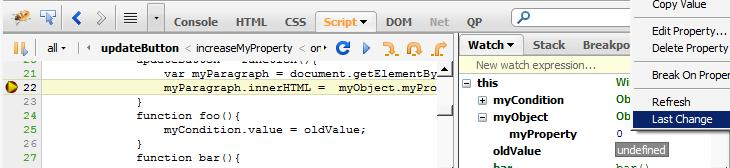
\includegraphics[width=1.0\textwidth,
    height=.17\textheight]{1-bp22.jpg}}

\subfigure[Developer can query \textit{lastChange} on a value by right-clicking 
on the
  value of \texttt{myProperty}.]{\label{fig:example2}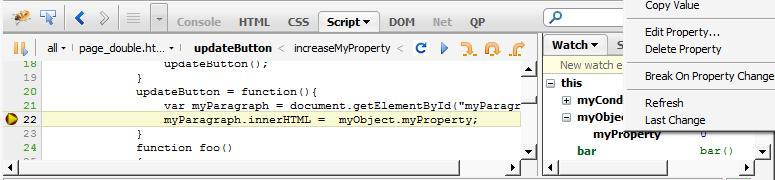
\includegraphics[width=1.0\textwidth,
    height=.17\textheight]{2-bp22-lastChange.jpg}}

\subfigure[The result of \textit{lastChange} query for
  \texttt{myObject.myProperty}. The left panel, QP, shows the source
  code at the point of \textit{lastChange}; The right panel,
  TraceData, shows the collected data at the
  point.]{\label{fig:example3}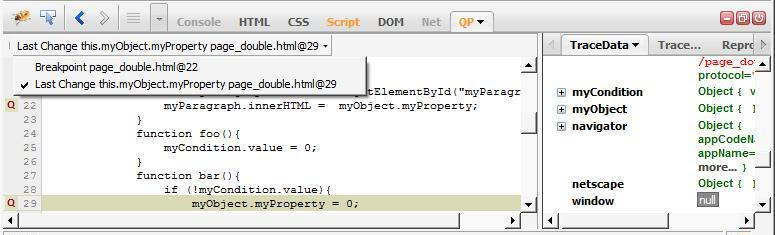
\includegraphics[width=1.0\textwidth,
    height=.21\textheight]{3-lastChange.jpg}}

\subfigure[The result of \textit{lastChange} query for
  \texttt{myCondition.value}. The opened list on the top of the left
  panel shows the visited execution points. Clicking on each point in
  the list shows the corresponding code and
  data.]{\label{fig:example4}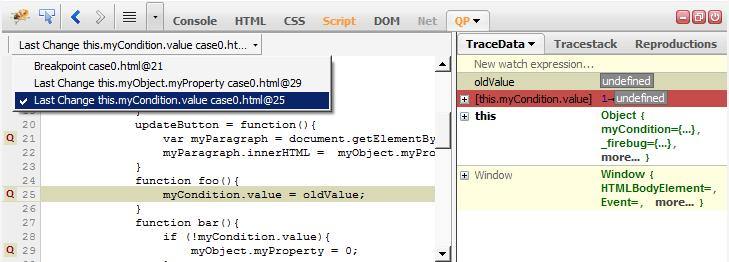
\includegraphics[width=1.0\textwidth,
    height=.23\textheight]{4-lastChange2.jpg}}

\caption{The stages of locating the defect using \textit{lastChange} feature.}
\label{fig:lastChange}
\end{figure*}


\begin{figure}[htp]
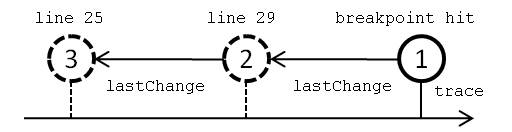
\includegraphics{5-example-points.jpg}
\caption{The examined points before locating the defect. The arrow represents the logical forward progress of the program. Three actual executions are superimposed on this arrow. All three stop at the reproduction point indicated by the circle 1. After the first execution, the developer asks for lastChange as described in \ref{sec:introExample}, yielding information  indicated by circle 2. After the second execution, another lastChange query causes a third execution, yielding information indicated by circle 3.}
\label{fig:example-points}
\end{figure}


Notice that in our example, \textit{lastChange} combines some aspects
of breakpoint and of log-based debugging. Like breakpoint debugging,
the developer re-executes a live runtime without changing the source
and without a special execution environment beyond the debugger. The
state of the program memory and the call stack are available at each
lastChange point. Like log-based debugging, the program state and the
call stack are recorded during program execution. We can't halt the
program at \textit{lastChange} because we don't know which point is the last
one until we return to the original breakpoint. (In section 5 we
discuss cases were it is possible to pause at lines of \textit{lastChange}).

\section{\textit{lastChange} Algorithm}

The \textit{lastChange} algorithm is based on program re-execution of
a program halted on a breakpoint. The algorithm starts when developer
examines the program state at a breakpoint hit and asks for the
\textit{lastChange} of a value. The breakpoint hit becomes the
\textit{reproduction point}. Debugger sets hooks (a callback
function dependent upon the underlying runtime) on all instructions
that might be the result of \textit{lastChange} query. Then the
debugger re-executes the program and every time a hook hits it
checks for a \textit{change event}. In the case of a change, it stores
part of the program state values.  Once the execution reaches the
reproduction point, it analyzes the collected data and shows the
result.  The program state at the execution point of the last change
event is the \textit{lastChange}.

As \textit{lastChange} itself is not a different kind of \textit{breakpoint},
all of the assumptions developers already have for breakpoints hold
for \textit{lastChange}. In particular the re-execution is just the
same operation developers use to debug with breakpoints. Because
\textit{lastChange} dramatically reduces the developers work in
setting and removing breakpoints, the re-execution step will become a
much larger fraction of the debug time. Therefore automatic mechanisms
for re-execution will be corresponding more valuable for debugging
with \textit{lastChange}.

As we described in the preceding section, a \textit{lastChange} query can
be performed on the result of another \textit{lastChange} query. If we
name the reproduction point \textit{R}, we can write the first
\textit{lastChange} in the introductory example in this form:
\textit{lastChange(R, myObject.myProperty)}. It means that this query
is defined at \textit{R}. If we name the result of this query
\textit{A}, we can write the second \textit{lastChange} in this form:
\textit{lastChange(A, myCondition.value)}. In this way, a sequence of
\textit{lastChange} queries with any length can be defined.

\textit{lastChange} can be called on two different types of values: An
object property or a variable value. Three different variations of the
algorithm are required, one for object property and two more depending
upon the scope of a variable.

\subsection{\textit{lastChange} on object property}
To simplify the algorithm explanation and defer technical details, we
define two basic operations and later we explain the details of these
two operations. The first operation is \texttt{objectId()}: given a
JavaScript object it returns an integer as its identifier. This
identifier is unique to the object during one execution.  By using an
object id instead of an object reference we allow the garbage
collector to reclaim the space for dead objects just as it would in the
absence of the debugger. The second
operation is \texttt{setPropertyChangeHook()}: given a function and a
string, the function is called whenever a property changes and its
name matches the string For example, if the is 
\texttt{foo} so changes to \texttt{bar.foo} or \texttt{baz.foo} would
call the function.  The callback function receives a reference to the
owner of \texttt{foo}. In the next section, we describe how we use
a slightly different version of this operation which is restricted 
to the created objects in one location instead of all objects.

To see how these functions work, suppose the developer asks for the
last change of \texttt{bar.foo} at the reproduction point in a
program. The debugger calls \texttt{setPropertyChangeHook()} with
\texttt{foo} as the property name and re-executes the
program. Whenever \texttt{foo} changes and the callback function is to
be called, debugger first calls \texttt{objectId()} on the
\texttt{foo} owner object. Then it stores this owner id, the stack
frame locations, and other state values in scope at the call point.
Whenever the execution reaches the reproduction point the debugger
looks at the history of \texttt{foo} changes and finds the last
\texttt{foo} change with the same object id as \texttt{bar} id at the
reproduction point. Figure ~\ref{fig:foo-changes1} shows the list of
property \texttt{foo} change events in a hypothetical
execution. \texttt{bar} id at the reproduction point is 1010, so the
last change of \texttt{bar.foo} is the fourth column. 

\begin{figure}[htp]
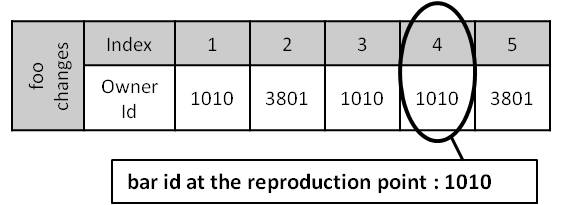
\includegraphics[width=.48\textwidth]{6-foo-changes1.jpg}
\caption{The list of property \texttt{foo} change events and
  \texttt{bar} id at the reproduction point which identifies the last
  change of \texttt{bar.foo} in the list. Column 3 is also a change of
  the object we want to study, id 1010, but it is not the last change;
  Column 5 is also a change of a property \texttt{foo} but its not for
  the object we are interested in.}
\label{fig:foo-changes1}
\end{figure}

\subsection{\textit{lastChange} on variable} 
In JavaScript, every frame has a scope chain and every available
variable in the frame comes from one of the scopes in the frame's
scope chain. Once a developer asks for the last change of a variable with name 
\texttt{foo} at the reproduction point, the debugger first determines the
variable's scope as follows: it iterates over the scopes in the scope
chain and the first scope which has a variable with the same name is
the variable's scope. There are five different scope types: local,
global, \texttt{with}, closure and \texttt{catch}. We explain these
cases in two groups.

\begin{figure}[htp]
\begin{verbatim}

  function f(){
    var x = 0;
    x++;
    if (!stop) f();
  }

Sample Trace:

   f()
A  |  x changes, scope 1 
   |  f()
   |  |  x changes, scope 2
   |  |  f()
B  |  |  |  x changes, scope 3 
C  |  ... , scope 1

\end{verbatim}
\caption{A recursive call trace demonstrates the need for scope
  id. In the absence of scope id, querying \textit{lastChange} on \texttt{x}
  at point C in scope 1 returns point B which is the last change of variable 
  \texttt{x} but happens in another scope. However, the right answer is point A
  which is in the same scope as point C.}
\label{fig:recursive}
\end{figure}

\subsubsection{global and \texttt{with} scopes}
Global scope is the the most outer scope in the scope chain and it is
also referred to as the global object (the \texttt{window}
object in Web pages). This scope is a regular JavaScript object and therefore every
global variable is a property of global object. Similarly,
 \texttt{with} scopes are also regular objects. A \texttt{with}
scope is created by a \texttt{with()} block with an object as the
parameter. Every property of this parameter object is available inside the
block as a variable. \textit{lastChange} treats the case where variable's scope
is global or \texttt{with}, like it does on an object
property.

\subsubsection{local, closure and \texttt{catch} scopes}
Local scope refers to the most nested scope in the scope
chain which contains the local variables. Closure scope refers to the 
scope which is created for a nested function and contains variables 
defined in the outer block. Catch scope is the scope created in the catch
block of try-catch statements and contains the exception
variable. These scopes are not necessarily regular JavaScript
objects. Scope object is usually a transient copy of a native object. 
Therefore, to track changes to a variable in these scopes we
employ a different approach.


Having the scope chain and the source code, we can map every scope to % perhaps needs more explanation, how?
a code block, enclosed the executing code. In
JavaScript, a code block can be identified by the file url and  
the block's first instruction program counter. Given this information, the debugger is
able to recognize the code block once it is loaded.
Similar to \textit{lastChange} on object property, we define two basic operations: 
\texttt{scopeId()} and \texttt{setVariableChangeHook()}. The first one, 
given a scope returns an integer as the scope's identifier. The second one, 
given a callback function, a code block and a variable name-
which is defined inside the block-, the function is called
whenever the variable is changed. Figure ~\ref{fig:recursive} demonstrates a case in which the same syntactically variable
\texttt{x} is changed several times but in different scopes due to the
recursive calls. Without considering the scopes calling \textit{lastChange(x)}
at point \texttt{C} in scope 1 will return point \texttt{B} which is a change of \texttt{x} in 
scope 2 while the right answer is point \texttt{A}. To resolve this issue, an id
is assigned to the scope by \texttt{ScopeId()} operation and the scope id is also stored 
at every variable change event.

If the developer asks for the last change of variable \texttt{foo} at the 
reproduction point in a program, debugger calls 
\texttt{setVariableChang-} \texttt{eHook()} with the variable's defining
block and name as parameters and re-executes the
program. Whenever \texttt{foo} changes and the callback function is to
be called, debugger first calls \texttt{scopeId()} on the
variable's scope. Then it stores this scope id, the stack
frame locations, and other state values in scope at the call point.
Whenever the execution reaches the reproduction point the debugger
looks at the history of \texttt{foo} changes and finds the last
\texttt{foo} change with the same scope id as the variable's scope id
at the reproduction point (Figure ~\ref{fig:foo-changes2}). 


\begin{figure}[htp]
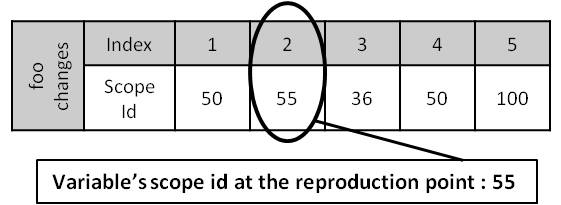
\includegraphics[width=.48\textwidth]{7-foo-changes2.jpg}
\caption{The list of variable \texttt{foo} change events and the
  \texttt{foo}'s scope id at the reproduction point which identifies
  the last change.}
\label{fig:foo-changes2}
\end{figure}

 
\subsection{\textit{lastChange} on \textit{lastChange}}
The algorithm we explained so far needs an enhancement to support
cascades of \textit{lastChange}s. We first explain the issue
and then the solution. Consider the following points:

\begin{center}
\textit{
 point A : the reproduction point \\
 point B : lastChange(A, bar.x) \\
 point C : lastChange(B, baz.y) 
 }
 \end{center}
According to the algorithm explained in the previous section
the points B and C cannot be identified before reaching point
A. That is, as execution moves through point B we cannot know it will be the point of last change until
we reach A, and we cannot apply the simple algorithm to look for point C until we know B. 
 Therefore, all \texttt{x} change events for point B and all \texttt{y}
change events for point C are stored. Once the execution reaches point A,
and the exact \texttt{bar} id reveals, point B can be identified among
the change events in the history of \texttt{x} changes. The problem
arises in recognizing point C. To recognize point C, we need
\texttt{baz} id at point B, but B is a past program state, and
\texttt{baz} id has not been collected at this point.

To address this issue, we use Algorithm \ref{dependency-analysis}, to
create the list of additional data (object id or scope id) should be collected at a change
event. This algorithm does a dependency analysis between all
\textit{lastChange} queries and computes the list of additional data
required to be collected at each change event. For example in the
mentioned case, \texttt{baz} id-if it is available- should be
collected at all points \texttt{x} changes. Having this additional
data, \texttt{baz} id at point B, it is enough to look at the list
of \texttt{y} changes and find the last change event with the same 
owner id (Figure ~\ref{fig:lastchange-lastchange}).

\begin{algorithm}
\caption{\textit{lastChange} queries dependency analysis.}
\label{dependency-analysis}
\begin{algorithmic}

\FOR{$q$ in $lastChange queries$} 
 \FOR {$p$ is defined at the $q$ result}
   \IF {$p$ is a lastChange on object property} 
     \STATE the property owner id should be stored at $q$ change events. 
   \ELSIF {$p$ is a lastChange on variable} 
     \STATE the variable scope id should be stored at $q$ change events.
	 \ENDIF 
 \ENDFOR 
\ENDFOR

\end{algorithmic}
\end{algorithm}

\begin{figure}[htp]
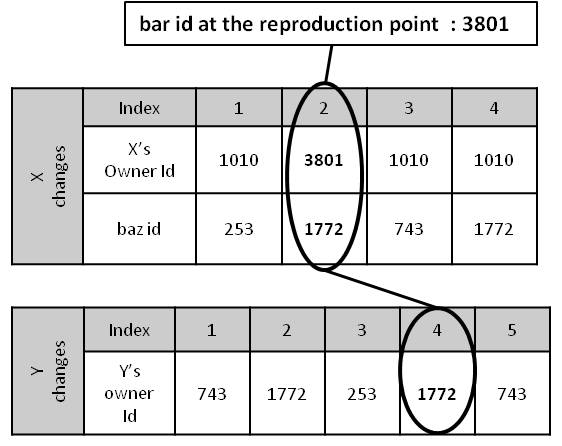
\includegraphics[width=.48\textwidth]{8-lastchange-lastchange.jpg}
\caption{The list of change events stored for locating point B, the
  \textit{lastChange} of \texttt{bar.x} at the reproduction point, and
  point C, the \textit{lastChange} of \texttt{baz.y} at point B.}
\label{fig:lastchange-lastchange}
\end{figure}



%---------------------------------------------------------------------------------------------------
\section{JavaScript implementation}
To verify the \textit{lastChange} algorithm we
implemented it in an extension to the Firebug
JavaScript debugger\cite{Firebug}. %\cite{firebug-version-1.6}. 
Firebug itself is an extension of the Firefox browser\cite{Firefox}. %\cite{firefox-version-3.6}
The Firefox JavaScript engine provides a JavaScript debugging interface \cite{JSD} and 
\textit{Querypoint} is developed over this interface. Our prototype implementation defines our four primitive operations in JavaScript code and using techniques which are cumbersome and comparatively slow to execute.  A professionally useful debugger would implement these primitive operations in the Javasript engine.

\subsection{\texttt{objectId()} operation}
\texttt{objectId(obj)} first checks the argument \texttt{obj} for a property \texttt{\_objectId}.
It returns the value if this property is already defined,
otherwise it generates a new id and sets this property. The value of the id is simply an integer incremented 
for each new \texttt{\_objectId} needed. To assign the id to the object we 
set the id as a regular object property. This might change
the program behaviour due to the appearance of this property in 
\texttt{for(property in object)} loops. \texttt{defineProperty} is a standard JavaScript
function which is available in the next version of Firefox\footnote[1]{https://developer.mozilla.org/en/JavaScript/Reference/Global\_Objects\\/Object/defineProperty}. \texttt{defineProperty} receives 
an argument which specifies whether the property is enumerable or not. By setting the enumerable
field \texttt{false} for \texttt{\_objectId}, this property will not
apear in \texttt{for(property in object)} loops and therfore has no
effect on the program execution. Note that \texttt{\_objectId} is
not set for all objects but only those objects that need an id.

\subsection{\texttt{setPropertyChangeHook()} operation}
The Firefox JavaScript engine supports watching property changes in an
object. Every object has a function \texttt{watch(propName, callback)}
which receives two parameters, a property name and function.  Whenever
the property with the given name changes, the \texttt{callback} function is
called. The hook set by this function remains enabled even if the
property is deleted and defined again. 

For our purposes, the \texttt{watch()} function only covers the case
of global object properties. At the beginning of execution, no object
excepting the global object is available.  For 
the our \textit{lastChange} prototype we created a version of
\texttt{setPropertyChangeHook()}.  The basic strategy is to get a reference to the object just
after its creation, then use \texttt{watch()} function to monitor
property changes in the object. Setting a flag\footnote[2]{DISABLE\_OBJECT\_TRACE defined in jsdIDebuggerService.idl} into the Firefox %\cite{JSD}
JavaScript engine we can get file URL and line number for each object
creation (e.g., myFile.js, line 24). We set a hook on this line
and analyze the source code to determine which object was created.

The only data we have is the object creation location including the
file url and the line number and the goal is to get a reference to
this object. Although in the most regular cases we have only one
statement and one object creation in a line, there are cases that more
than one object might be created in a line. There is no way to
recognize the interesting object among these new objects. So instead
of one object, we monitor all new objects created in the line.

An object might be created by one of these statements: object
initializer (\texttt{\{...\}}), \textit{new} operator (\texttt{new 
constructor()}) or function definition statment (\texttt{function()}). 
By parsing the source code we can recognize the statements that
create an object. The next step is getting a reference to the new object.

The new object can be assigned to an object property or a variable by
an assignment (\texttt{=}). In these cases we keep the assignee statement 
at the left side. The idea is that we create a list of assignee statements 
that the new objects are assigned to. We set a hook on the creation
line. Once the hook hits, we evaluate all assignee statements. Then 
we do stepping(step-over) and after each step we evaluate the
statements. Every statement which has a new value, we consider the new
value-if it is an object-as a new object. For example in Figure
~\ref{fig:objectCreation}(a), if the creation line number is 20, we
have only one statement which creates a new object and it is assigned
to \texttt{x.y}.


The new object can also be set as the property of a parent object by a
colon (\texttt{:}). This case is also treated similar to previous case. The
only difference is that the full path of property from the root parent
in the local scope should be considered as the assignee statement. For
example in Figure~\ref{fig:objectCreation}(b), if the creation line
is 20, we keep \texttt{parentObject.newObject}. In this case stepping
should be continued until the end of line 22 for getting a reference
to the created new object.

There is another case for new objects and when they are passed as
arguments to other functions (Figure~\ref{fig:objectCreation}(c)). In these
cases instead of step-over we use step-in and we get the corresponding
argument as a new object.

Although this approach is successful in many ordinary cases, there are some 
cases where this approach doesn't work. For example in a case
where the new object is assigned to \texttt{a[++i]} where i is a variable
(Figure ~\ref{fig:objectCreation}(d)), \texttt{a[++i]} is kept in the list
of assignee statements. Obviously, evaluating this statement doesn't return
a reference to the new object. Our prototype implementation does not handle these kinds of unusual cases yet.

Throughout this section we implicitly assumed that the object will be created at 
the same location in the next execution. So, what does happens if it
is not true? Well, once the execution reaches the reproduction point, it
reveals that the object has been created in different location. This time,
debugger re-executes the program considering both locations as possible 
object creation locations.


\begin{figure}[htp]
\begin{verbatim}
(a) Case 1:
20 x.y = new myConstructor();

(b) Case 2:
19  parentObject = {
20   	  newObject : {
21  			x : 5
22  }}

(c) Case 3:
20 myFunction({myProperty:5});

(d) Case 4:
20 a[++i] = new myConstructor();
 
\end{verbatim}
\caption{Examples of three types of JavaScript object creatin statements.}
\label{fig:objectCreation}
\end{figure}

\subsection{\texttt{scopeId()} operation}
The debugger sets a hook at the beginning of all code blocks needing
a scope id. The scope id is kept as a variable with name 
\texttt{\_scopeId} in the scope. Whenever the hook is hit,  meaning a new scope
is created, \texttt{\_scopeId} is set by calling JavaScript's dynamic compilation 
function \texttt{eval()}. For example, executing \texttt{eval( var \_scopeId = 10)} creates a
variable with name \texttt{\_scopeId} and value \texttt{10} in the
scope of the \texttt{eval()} call, which is our interesting scope. \texttt{scopeId()}
operation returns the value of \texttt{\_scopeId} in the scope.

\subsection{\texttt{setVariableChangeHook()} operation}
Variables defined in local, closure, and catch scopes are only changed in
their scope; that includes the defining scope and scopes nested whithin them.
For example in Figure ~\ref{fig:js-closure}, variable \texttt{var1} in line 11 can only be
changed in lines 10 to 23. Therefore, after locating the function in
which the variable is defined, it is enough to parse the code inside
the function block and set a hook on all lines where the variable is
assigned a new value. 
We also set a hook at the first line of the function which is
corresponding to the line where the variable is defined. In Figure
~\ref{fig:js-closure}, if the execution is paused at line 17 and the
last change of \texttt{var1} is queried, two hooks on lines 16 and 17
will be set, but if the execution is paused at line 20 , four hooks on
lines 11, 12, 14, 20 will be set. These two cases are different due
the fact that \texttt{var1} in \texttt{firstChild} is a local variable
but in \texttt{secondChild} is a closure variable.

\begin{figure}[htp]
\begin{verbatim}
10  function parent(){
11    var var1;
12    var1 = ...;
13    function myfun(){
14      var1 = ...;
15      function firstChild(){
16       	var var1;
17        var1 = ...;
18      }  
19      function secondChild(){
20        var1 = ...;			      
21      }
22    }  
23  }    
\end{verbatim}
\caption{Sample JavaScript code demonstrating local and clousure variables.}
\label{fig:js-closure}
\end{figure}

\subsection{Re-Execution, reproduction point and data collection}
\textit{Querypoint} needs a test case to reproduce the
execution and conditions to correctly recognize the reproduction point. 
Although both elements can be directly provided by developer, \textit{Querypoint}
is also able to automatically create them from the first execution. 

\textit{Querypoint} keeps track of breakpoint hits and single steps. For example, 
if the developer queries \textit{lastChange} at the third hit of breakpoint \textit{b}, in
re-execution, the third hit is recognized as the reproduction point. 

To build a test case from one execution, two elements should be carefully 
considered. First, the initial state should be the same as the initial state
of execution. Second, similar actions and events should be applied to
the program during the execution. \textit{Querypoint} supports two mechanism
for automatic re-execution: local-reproduction, record-replay. The first one,
recalls the function at the bottom of the call stack with the same parameters. The idea
behind this mechanism is that many bugs in web pages can be reproduced by firing
an event like clicking on a button. The second one, in the first execution, record phase, 
stores the initial page url and captures user actions. In the replay phase, it opens
the same url and applies user actions. The local reproduction mechanism provides
shorter re-execution cycles while the record-replay is more accurate about the
initial state.

In addition to the data collected at every change event for identifying the \textit{lastChange}
result, \textit{Querypoint} partially stores values in program state. If developer asks for 
some values which have not been stored, \textit{Querypoint} re-executes and collects the requested data.
There is a trade-off between the amount of data collected at every change event and the number of re-executions. 
By default, \textit{Querypoint} stores values up to one level depth in objects.



% Discuss what happens when assumptions changes, like object creation location.

\section{Reproducible Non-deterministic Execution}

By construction \textit{lastChange} works whenever conventional
breakpoint debugging works. By that we mean that, since we use
conventional breakpoint debugging technology under the covers,
\textit{lastChange} works whenever breakpoint debugging
works. However, there are cases where breakpoint debugging fails but
\textit{lastChange} works.  These are cases of \textit{reproducible
  non-deterministic} execution.

A bug is \textit{reproducible} for a developer when the developer can
start from a determined initial state, operate on the program with a
list of actions, and reproduce the symptoms of the bug. The details of
the execution can change each time we re-execute the buggy program,
but the buggy result is the same.  The reproducibility of the bug
means that the defect is very unlikely to depend on the order of
events during the execution. When the developer selects a value and
asks for \textit{lastChange}, they are expressing an hypothesis that
the value is related to the defect. Therefore the reproducibility of
the bug makes it very unlikely that the \textit{lastChange} will
depend upon order of events during execution.

Since \textit{lastChange} does not rely on determinism, some bugs that
confound breakpoint debuggers will be easier to find with
\textit{lastChange}.  Consider the example in 
Figure ~\ref{fig:counter-example}. It shows a function which processes an
array. The array contains numbers except one item which is
\texttt{undefined} and it causes a bug in line 30. There is a call to
\texttt{randomPermutation} function in line 11 which randomly
permutes the array item. So at every execution the
\texttt{undefined} item will be in a new place. Calling
\textit{lastChange} on \texttt{x} at the place bug happens, gives a
point which shows line 14. Although this point exists at every
re-execution but it can not be identified by a conditional breakpoint.

\begin{figure}[htp]
\begin{verbatim}
10 function randomProcess(array){
11   randomPermutation(array);
12   var x, y;
13   for (var i=0 ; i<array.length ; i++){
14      x = array[i]
...
30      y = x+1;
31   }
32 }
\end{verbatim}
\caption{A counter-example for transforming \textit{lastChange} to a conditional breakpoint.}
\label{fig:counter-example}
\end{figure}
 

Thus in the case of a non-deterministic program, a \textit{lastChange}
is not equivalent to any series of conventional watchpoints or
breakpoints. The extra power of \textit{lastChange} derives from its
analysis of the entire execution up to the reproduction point and its
memory of previous work on the defect.  Each time we re-execute a
non-deterministic program, the details of execution instruction order
may change. For example, if we record the source code lines every time
a conventional watchpoint hits, the record may differ each time we
re-execute. But \textit{lastChange} does not ask the developer to
consider these single points.  Rather we analyze all of the
watchpoints in an entire execution at the reproduction point where we
know the defect has already occurred and only show the final result to
the developer.

Of course there can be cases where the defect is reproducible but the
value from \textit{lastChange} is not. As in conventional breakpoint
debugging, we can only determine this empirically, by observing
multiple executions with different values. Unlike conventional
breakpoint debugging, implementations of \textit{lastChange} readily
aid in detecting such cases: as we work back through a series of
\textit{lastChange} requests we can compare values with previous
executions. Different values on different executions will signal that
the execution is not deterministic. In future we hope to compare
queries from successive executions as a tool for learning about
non-deterministic executions.

%\subsection{Reproduction point}

\section{Discussion}

We have presented the \textit{lastChange} algorithm and describe our
prototype implementation. Now we want to convince you that the
algorithm has practical value. Ultimately, practical value can only be
proven by developers in the field using the technique. This paper is
one step to convince implementers to put \textit{lastChange} in the
field.  Thus our goal here is a persuasive argument for potential implementors.

The key ingredients in our argument are: 
\begin{enumerate}
   \item developers need an operation like \textit{lastChange}, 
   \item developers can learn to use \textit{lastChange}, 
   \item practical implementations are feasible with modest
invested development time,
   \item in most cases \textit{lastChange} will be much faster than current alternatives,
   \item the worst cases are not more common or more painful than
alternatives.
\end{enumerate}

\subsection{Developers need an operation like \protect\textit{lastChange} }

We have shown how \textit{lastChange} identifies the prior point in
program execution where a program state value changes. Is it something
the developer needs to do?  Since ultimately programs are just
transformation of state values, debugging is ultimately backtracking
to find defects in program state change.  When a developer halts a
program on a breakpoint they have three kinds of information: a model
of the program in their head, a call stack showing what part of the
program is halted, and the state at that point (a combination of the
debugger's view of the program internal state and the output of the
program up to this point of execution). If the model does not match
the call stack or if no value in the viewable program state aligns
with the developers model for this point in execution, the developer
will seek another view by changing the breakpoint or the input
data. If a value appears incorrect, they may have a flash of insight
and know the defect. Otherwise they need to figure out what operation
causes the incorrect value. Here \textit{lastChange} takes over and addresses a key
part of the debugging process.

\subsection{Developers can learn to use \protect\texttt{lastChange}}

If \texttt{lastChange} could be useful, can developers figure out how
to use it? We hope that our prototype demonstrates that
\textit{lastChange} can be easily activated by operations on the
graphical representation of erroneous data in a debugger. Interpreting
the results should be only slightly more difficult. We designed the
user interface for the results from \textit{lastChange} to resemble
the results from a breakpoint, with the source code of the change
point highlighted and the state of the program presented the way state
is presented from a breakpoint. Based on this user interface, we
believe developers can start to use \textit{lastChange} with minimal
training. Of course developers may initially confuse the result of
\textit{lastChange} with being halted in a debugger at the point of
last change. The value of the result will motivate them to clarify the
issue.

\subsection{Practical implementations are feasible}

We described our prototype implementation in Sec. 4. A fully usable
implementation would require access to the object id at the point of
object creation and \texttt{setPropertyChangeHook()}. Many
object-oriented runtimes provide object identifiers[] and some
provide access to object creation[]. In the particular case of
the Firefox Web browser we used for our prototype, the primary barrier
to practical implementation would likely be integration with the
increasingly sophisticated just in time compilers []. In the case of
tracking variable changes, \texttt{setVariableChangeHook()} can be implemented
similar to \texttt{setPropertyChangeHook()} if JavaScript scopes-like regular 
JavaScript objects-support \texttt{watch()} function.

\subsection{In most cases \protect\texttt{lastChange} will be much faster than current alternatives}
When developers try \textit{lastChange}, will they get results fast
enough to benefit? While we only used our prototype on toy programs,
\textit{lastChange} seemed as fast as re-execution.  Recall that we
insert additional code through debugger callbacks, then re-execute the
program. The additional code we insert is proportional (in our
JavaScript algorithm) to 1) the number of places a property or
variable with a given name is changed, 2) the number of places objects
are created. (Something about the likely overhead in Firefox).

For comparison we should use the practical alternative: developers
setting breakpoints. For the vast majority of programs, a developer
will take much more time to set one breakpoint than
\textit{lastChange} would add. But typically the developer may not
guess the point of last change. They must then ponder another
breakpoint, and re-execution. 

We could also compare to solutions based on logging or tracing. Manual
logging has very high overhead: the developer must add code, debug
that added code, then analyze the log. (To be fair, the log can become
a permanent debugging aid.) Automatic logging as we discussion in
\ref{sec:relatedWork} causes about one or two orders of magnitude slow down. 

\subsection{The worst cases are not more common or more painful than alternatives}

Finally we consider the worst cases: what about code that changes
objects in long running loops? Every time through the loop we incur
the call back overhead; if the loop itself has relatively little code
the overhead could be very large; if the loop computation is a
significant fraction of the full program, the slowdown would be
enormous. 

Of course breakpoints are not feasible in these cases and logging
becomes unwieldy. Since automatic logging solutions are highly tuned,
their overhead in this case will likely be much less than
\textit{lastChange}. On the other hand, \textit{lastChange} integrates
with an interactive debugger and detecting that we are in a high
overhead loop is simply a matter of checking our internal counter. In
such unusual cases we may simply offer the developer the option of
studying the loop code then omitting it from \textit{lastChange}
operations. As a practical result, this is no different from similar
issues developers face with any debugger today: occasionally a
debugger causes too much overhead to be useful for debugging. On
balance we think \textit{lastChange} will rarely encounter these kinds
of issues.


%\section{Evaluation}
%\subsection{\textit{lastChange} effectiveness}
%\subsection{Execution overhead analysis}

%If we assume that the total number of instructions in an execution is
%$n$ and $m$ change event happens during one execution and for every
%change event $k$ additional instructions should be executed, the
%execution overhead of our approach is $mk/n$. For $m=10^3$, $k=10^2$
%and $n=10^{10}$ the overhead is very low and about $10^{-5}$.

\section{Related Work}
\label{sec:relatedWork}

\textit{lastChange} functionality supports obtaining information about
the execution state logically earlier in the control flow. This
support resembles a mixture of replay-based and logging-based
debugging. Replay-based approaches capture limited data during
execution and replay the buggy execution to reach past points. In
contrast, logging-based approaches collect enough data during
execution to relieve developer from re-execution. Replay-based
approaches impose much less runtime overhead (about two orders of
magnitudes) comparing to logging-based approaches. However, developer
has to re-execute the buggy execution several
times. \textit{lastChange} functionality collects data on re-execution
but this data is limited to the current queries of developer.

Among replay-based debuggers we compare to bdb \cite{Boothe} and
reverse watchpoint \cite{Maruyama}.  A bidirectional C debugger, bdb
employs a step counter to locate the requested point from the
beginning of execution. It relies on deterministic execution replay
(i.e., the same sequence of instructions in re-execution) and records
the results of non-deterministic system calls and re-injects them into
the program when it is replayed. It makes use of checkpoints to reduce
the time needed for re-execution.  Reverse watchpoint, is proposed by
Maruyama et al., analyses the execution and moves the debugger to the
last write access of a selected variable by re-executing the program
from the beginning\cite{Maruyama}.  Similar to bdb it relies on deterministic
replay and uses a counter to correctly locate a point in the next
execution. The main disadvantage of these approaches is requiring the
exactly the same executions. Even one instruction difference between
two executions leads to wrong results. On the other hand,
\textit{lastChange} doesn't require any special feature in the
re-execution and it is fit to  developers' everyday debugging
practice.

Among logging-based approaches are \textit{omniscient} debuggers
ODB\cite{Lewis} and Unstuck\cite{Hofer}. Both
approaches keep the log history in memory and hence can only record
and store the complete history for a short period of time. These
debuggers record all the events that occur during the buggy execution
and later let the developer to navigate through the obtained execution
log. In this approach there is no execution to resume: moving
backwards in the log can be similar to moving forwards. Omniscient
debuggers suffer from a different set of issues. First, the recording
step is time expensive and it should be repeated in case of changes in
program. Second, the execution log cannot fully replace the live
execution. There are other aspects of execution (e.g., program user
interface, file system, database tables, etc.) which are also
important in debugging and are not available to the developer in
omniscient debuggers. Third, querying collected data (e.g., to restore
the program state at a certain point) may not be efficient enough for
debugging of realistic programs.

A more scalable approach has been proposed by Pothier et
al. \cite{Pothier}. Their back-in-time debugger, TOD, addresses the
space problem by storing execution events in a distributed
database. Comparing to Omniscient debuggers our approach is
lightweight and more flexible. Developer can start debugging just
after reproducing bug without a capturing step.  Changing inputs or
environment settings and re-executing to investigate the bug works as
in conventional breakpoint debuggers.

A recent work by Lienhard et al.\cite{Lienhard} suggests virtual
machine level support for keeping the object flow. It replaces every
object reference with an alias object which keeps the history of
changes to the object reference. In this way, when an object is
collected by garbage collector, its track of changes (if it is not
referenced by other aliases) will be also collected. Though this
approach incurs less runtime overhead (7 times to 115 times) in
comparison to omniscient debuggers, it adds memory
overhead. 

Origin tracking of undefined and null values employing \textit{value piggybacking} technique proposed by
Bond et al. \cite{Bond}. This approach has two main limitations comparing to \textit{lastChange}.
First, it is limited to undefined and null values. Second, this approach dosen't return the last change
of a null variable but the first place that the null value is originated.

Two new directions in logging debuggers explore more detailed use of
the log and more effective logging approaches. WhyLine\cite{Ko}
provides visual interface to collected runtime information and let
developer to move on execution log using queries expressed in terms of
the programming objects. WhyLine stores the program user interface in
addition to program trace and provides answers to why and why not
questions to the user. Jive\cite{Czyz} depicts the history of
execution by a sequence diagram and lets user to query on events
database. Both tools suffer from the requirement of gathering tracing information before their unique capabilities can be used.
We imagine that the runtime queries we use in \textit{lastChange}  may be used to gather data incrementally for these kinds of debugging approaches.



%Querypoint debugging uses re-executions to gather infor-mation requested by the developer: the memory overhead depends on the query not the entire program. Moreover, the Lienhard et al. debugger significantly changes the virtual machine, while our approach is a generalization to conditional breakpoints and available debugger infrastructure can be adapted to support it.
 
%\textit{lastChange} functionality does rely on a conventional breakpoint to begin queries, a requirement not shared by full logging solutions.  Here we leverage past experience of developers, but there are also new tools [] to help with this problem in the case of graphical and event based systems.


\section{Conclusion}
\textit{lastChange} provides critical information for debugging programs: the location and state at the point where a questionable value was assigned. It builds upon existing technology and developer experience making it a practical solution for implementers. Our prototype demonstrates the feasibility of \textit{lastChange} and its user interface hints at the potential this approach can have in organizing the debugging experience. 


% We recommend abbrvnat bibliography style.

\bibliographystyle{abbrvnat}

% The bibliography should be embedded for final submission.

\begin{thebibliography}{16}
\softraggedright

\bibitem[Bond(2007)]{Bond}
M.D. Bond, N. Nethercote, S.W. Kent, S.Z. Guyer, and K.S. McKinley. \newblock Tracking bad apples: reporting the origin of null and undefined value errors.
\newblock In \emph{22nd annual ACM SIGPLAN conference on Object-oriented programming, systems, languages, and applications(OOPSLA)},
October, 2007.

\bibitem[Bond(2010)]{Bond2}
M.D. Bond, G.Z. Baker, S.Z. Guyer, and Z. Samuel. \newblock Breadcrumbs: efficient context sensitivity for dynamic bug detection analyses.
\newblock In \emph{Conference on Programming Language Design and Implementation(PLDI)},
June, 2010.

\bibitem[Boothe(2000)]{Boothe}
B. Boothe. \newblock Efficient algorithms for bidirectional debugging.
\newblock In \emph{Conference on Programming Language Design and Implementation(PLDI)},
June, 2000.

\bibitem[Czyz(2007)]{Czyz}
J.K. Czyz, and B. Jayaraman. \newblock Declarative and visual debugging in Eclipse.
\newblock In \emph{OOPSLA workshop on eclipse technology eXchange},
October, 2007.

\bibitem[Firebug(2010)]{Firebug}
Firebug. \newblock http://getfirebug.com.

\bibitem[Firefox(2010)]{Firefox}
Firefox. \newblock http://www.mozilla.com.

\bibitem[Hofer(2006)]{Hofer}
C. Hofer, M. Denker, and S. Ducasse. \newblock Implementing a backward-in-time debugger.
\newblock In Proceedings of\emph{NODe'06},
volume P-88, pages 17-32. Lecture Notes in Informatics, 2006.

\bibitem[Ko(2008)]{Ko}
A.J. Ko, and B.A. Myers. \newblock Debugging reinvented: asking and answering why and why not questions about program behavior.
\newblock In \emph{30th international conference on Software engineering(ICSE)},
May, 2008.

\bibitem[LaToza(2006)]{LaToza}
T.D. LaToza, G. Venolia, and R. DeLine. \newblock Maintaining mental models: a study of developer work habits
\newblock In \emph{28th international conference on Software engineering(ICSE)},
May, 2006.

\bibitem[Lewis(2003)]{Lewis}
B. Lewis, and M. Ducasse. \newblock Using events to debug Java programs backwards in time.
\newblock In \emph{Companion of the 18th annual ACM SIGPLAN conference on Object-oriented programming, systems, languages, and applications(OOPSLA)},
2003.

\bibitem[Lienhard(2008)]{Lienhard}
A. Lienhard, T. G\^{\i}rba, and O. Nierstrasz. \newblock Practical Object-Oriented Back-in-Time Debugging.
\newblock In \emph{22nd European conference on Object-Oriented Programming(ECOOP)},
July, 2008.

\bibitem[Maruyama(2003)]{Maruyama}
K. Maruyama, and T. Kazutaka. \newblock Debugging with Reverse Watchpoint.
\newblock In \emph{Proceedings of the Third International Conference on Quality Software},
2003.

\bibitem[JSD(2010)]{JSD}
Mozila JavaScript Debugging Interface. \newblock http://www.mozilla.org/js/jsd.

\bibitem[Pothier(2007)]{Pothier}
G. Pothier, \'{E}. Tanter, and J. Piquer. \newblock Scalable omniscient debugging.
\newblock In \emph{22nd annual ACM SIGPLAN conference on Object-oriented programming, systems, languages, and applications(OOPSLA)},
October, 2007.


\end{thebibliography}

\end{document}
